\section{The ALERT Framework}
\label{sec:framework}
We present ALERT, a goal-conditioned agentic framework for proactive legal risk intelligence.
\subsection{System Overview}

Figure~\ref{fig:alert_arch} presents the architecture: a lightweight sensing pipeline populates evidence records, while the agentic layer plans, retrieves, verifies, and reports under a deterministic Goal Checker. The figure is included to show where the proposed retrieval-time authority gate enters the evidence path, not to claim novelty for the surrounding integrations.



\begin{figure}[t]
\centering
\resizebox{\linewidth}{!}{%
\begin{tikzpicture}[
  font=\footnotesize,
  box/.style={rectangle, rounded corners=2pt, draw, minimum height=0.56cm,
              align=center, inner sep=3pt, text width=2.05cm, line width=0.5pt},
  pipe/.style={box, fill=black!5, draw=black!55},
  agent/.style={box, fill=blue!8, draw=blue!55},
  outbox/.style={rectangle, rounded corners=2pt, draw=green!50!black, fill=green!10,
              align=center, inner sep=4pt, minimum height=0.55cm, text width=6.4cm, line width=0.5pt},
  arr/.style={-{Latex[length=1.4mm]}, draw=black!70, line width=0.5pt},
  lbl/.style={font=\scriptsize\itshape, text=black!55},
  grplab/.style={font=\scriptsize\bfseries, text=black!60}
]
% ---- left: sensing pipeline ----
\node[pipe] (ds) {Data Sources\\[-1pt]{\tiny CourtListener/RECAP $\cdot$ News}};
\node[pipe, below=0.22cm of ds] (sp) {Detect $\cdot$ Collect};
\node[pipe, below=0.22cm of sp] (sc) {Schema\\[-1pt]{\ttfamily\resizebox{1.85cm}{!}{ai-suit-sensing.csv}}};
\draw[arr] (ds) -- (sp);
\draw[arr] (sp) -- (sc);
% ---- right: agentic layer ----
\node[agent, right=2.0cm of ds] (pl) {Planner};
\node[agent, below=0.20cm of pl] (rt) {Retriever\\[-1pt]{\tiny LegalRisk-RAG}};
\node[agent, below=0.20cm of rt] (an) {Analyzer\\[-1pt]{\tiny Risk Scoring}};
\node[agent, below=0.20cm of an] (rp) {Reporter};
\node[agent, below=0.20cm of rp] (gc) {Goal Checker};
\draw[arr] (pl) -- (rt);
\draw[arr] (rt) -- (an);
\draw[arr] (an) -- (rp);
\draw[arr] (rp) -- (gc);
% schema feeds the agentic layer
\draw[arr] (sc.east) -- ($(sc.east)+(0.55,0)$) |- (pl.west) node[lbl, pos=0.72, above]{CSV};
% refine loop (Goal Checker -> Planner)
\draw[arr, draw=blue!60] (gc.east) -- ($(gc.east)+(0.62,0)$) |- (pl.east)
      node[lbl, text=blue!60, pos=0.25, right]{refine};
% ---- outputs ----
\node[outbox, below=0.42cm of $(sc)!0.5!(gc)$] (op) {Outputs: GitHub Issues $\cdot$ Slack};
\draw[arr] (gc.south) |- (op.north);
% ---- group containers ----
\begin{scope}[on background layer]
  \node[draw=black!35, dashed, rounded corners=3pt, inner sep=6pt, fit=(ds)(sp)(sc)] (gpipe) {};
  \node[draw=blue!40, dashed, rounded corners=3pt, inner sep=6pt, fit=(pl)(rt)(an)(rp)(gc)] (gag) {};
\end{scope}
\node[grplab, above=1pt of gpipe.north] {Sensing Pipeline (\texttt{ai-suit-tracker})};
\node[grplab, text=blue!55, above=1pt of gag.north] {Agentic Layer};
\end{tikzpicture}%
}
\caption{ALERT architecture. The sensing pipeline (left) detects filings, collects documents, and populates the schema; the agentic layer (right) plans, retrieves time-valid precedent, scores risk, and reports, with the Goal Checker driving a refine loop until evidence coverage is met.}
\label{fig:alert_arch}
\end{figure}

\subsection{Multi-Source Litigation Discovery and Schema Population}
\label{sec:discovery}

ALERT's discovery layer ingests CourtListener/RECAP~\citep{courtlistener2023}, docket-backed legal-media signals, and keyword-filtered news. A two-stage deduplication module first matches docket IDs and titles, then optionally removes Gemini-embedding neighbors above cosine $0.85$ (Algorithm~\ref{alg:hybrid_dedup}, appendix). Detected filings populate the 22-field \texttt{ai-suit-sensing.csv} schema by combining docket metadata, NER over complaint text, regex extraction for damages, and LLM summarization for the narrative fields.

\subsection{LegalRisk-RAG}

The LegalRisk-RAG pipeline adapts standard RAG to legal text in three ways. \textbf{Chunking} segments documents at \emph{logical structural boundaries}---numbered claims, ``WHEREFORE'' clauses, section headings---rather than fixed token windows, and each chunk retains a metadata header (case id, filing date, court level, section type). \textbf{Embedding}: we compared a dense retriever~\citep{karpukhin2020dense} (\texttt{text-embedding-3-large}), RECAP-tuned LegalBERT~\citep{chalkidis2020legalbert}, and a hybrid BM25 + neural re-ranker on a 200-pair development set; the hybrid (best) is the default (Table~\ref{tab:retriever_ablation}, appendix). \textbf{Dynamic context expansion (precedent chaining)}: when a retrieved chunk references a prior case (e.g., \emph{Authors Guild v.\ Google}), the pipeline appends that opinion as secondary context and queries the temporal precedent graph for subsequent treatment, so the Analyzer receives both semantic neighbors and validity metadata (cited positively, narrowed, superseded, or overruled at the filing date).

\subsection{Goal-Conditioned Agentic Loop}
\label{sec:agentic_loop}

The four specialized agents and the central Goal Checker operate as in Algorithm~\ref{alg:alert_loop}. The \textbf{Planner} decomposes unmet sub-goals into ordered retrieval/analysis sub-tasks; the \textbf{Retriever} runs LegalRisk-RAG queries and reformulates via legal entity term expansion when $\mathcal{G}_{\text{evidence}}$ is unmet; the \textbf{Analyzer} computes $\text{RiskScore}(d_i, P, C)$, clusters evidence, and maps clusters to a risk taxonomy (Training Data, Output Reproduction, API Misuse, Model Weights); the \textbf{Goal Checker} evaluates $\mathcal{G}(R_t)$ after each pass and returns machine-readable residuals such as \texttt{missing(valid-authority, DMCA, output-CMI, NDCA, 2025-02)}; the Planner converts these critiques into expanded entity/date/theory queries; and the \textbf{Reporter} assembles the risk register, per-risk evidence with citations, and mitigation guidance. The ingestion and risk-scoring components are released as \texttt{ai-suit-tracker} (anonymous review URL in the supplement), with configuration, prompt templates, and run parameters in the appendix.

\subsection{Supersession-Aware Temporal Precedent Graph}
\label{sec:tpg}

ALERT's central reusable mechanism is a retrieval-time authority gate implemented by a temporal precedent graph $\mathcal{P}_t=(V,E_t)$. Each node $v\in V$ denotes a case, order, or doctrinal rule and stores jurisdiction, court level, issue tags, filing/decision dates, and a validity interval $[s_v,e_v)$, where $e_v$ is open unless the node is later vacated, overruled, superseded, or materially narrowed. Directed edges encode treatment relations: \textsc{cites}, \textsc{distinguishes}, \textsc{narrows}, \textsc{supersedes}, and \textsc{overrules}. Retrieval for a query at date $t_q$ first obtains semantically relevant candidates and then applies validity gating:
\begin{equation}
\label{eq:tpg_score}
  \mathrm{score}(v,q,t_q)=\mathrm{sim}(v,q)\cdot \mathbf{1}[s_v\!\le\! t_q\!<\! e_v]\cdot w(\mathrm{treat}(v,t_q)).
\end{equation}
Here $w(\cdot)$ is a fixed, bounded monotone schedule in $(0,1]$: positively treated or still-open precedents take weight $1$, cautionary or materially narrowed authorities are down-weighted, and fully closed authorities are already removed by the indicator (the exact schedule is released with the implementation). This separates legal authority from topical similarity: a stale but lexically close case may be retrieved for context, but it cannot dominate the risk decision without passing the time-validity check. Algorithmically, Eq.~\eqref{eq:tpg_score} is a constrained retrieval operator over $(q,t_q)$, not a post-hoc explanation: it projects validity intervals onto the candidate distribution before entailment. Thus a host retriever may score semantic relevance normally, but PLRE receives only support whose legal status is operative at $t_q$. This differs from temporal features in a reranker, which can still rank closed authority highly, and from citator-style warnings, which occur after evidence selection.

\begin{figure}[t]
\centering
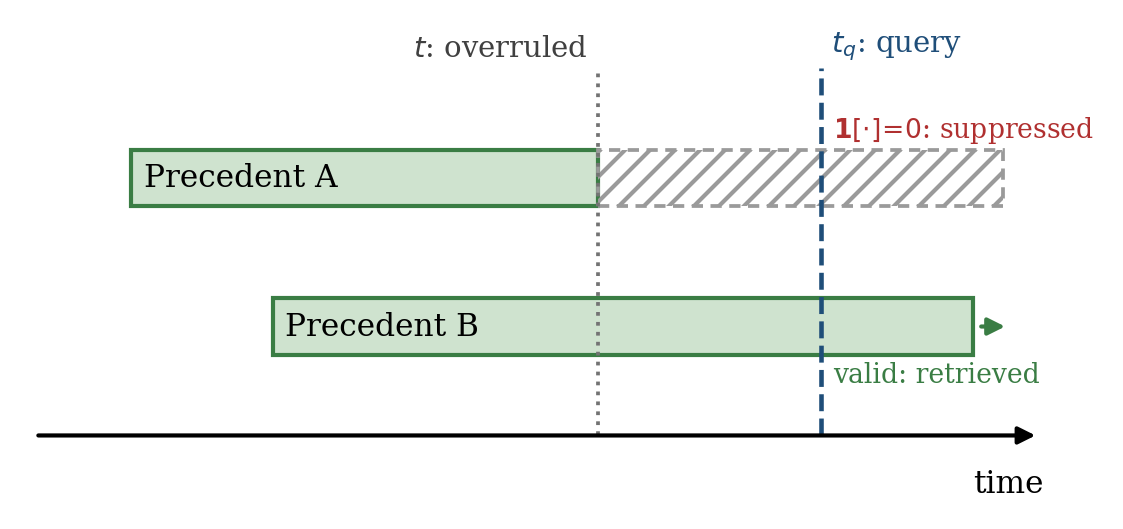
\includegraphics[width=0.99\linewidth]{fig_tpg.png}
\caption{Validity gating (Eq.~\eqref{eq:tpg_score}). An overruling at $t$ closes Precedent~A, so a query at $t_q\!>\!t$ zeroes its indicator and suppresses it despite lexical similarity, while still-open Precedent~B is retrieved---the time-valid distinction the RQ3 ablation isolates.}
\label{fig:tpg_mech}
\end{figure}

\paragraph{Graph construction and contamination controls.} The graph is built in three stages. \emph{Node induction}: each case, order, or rule from CourtListener/RECAP becomes a node with filing/decision dates from docket metadata and validity interval initialized to $[s_v,\infty)$. \emph{Edge extraction}: treatment relations are extracted from opinion text by a two-pass procedure---a citation-sentence detector locates candidate treatment spans, and an LLM classifier (GPT-4o, $T{=}0$, few-shot) labels the relation and polarity. To avoid self-contamination from generated legal conclusions, LLM outputs are treated only as candidate relation labels: interval-closing edges must be anchored to a detected citation span, docket/decision date, and source document identifier, and gold-set evaluation is performed on citation spans that were not used in prompt examples. \emph{Interval closure}: a confirmed incoming \textsc{overrules}/\textsc{supersedes}/material-\textsc{narrows} edge at date $t$ closes the target interval ($e_v\!\leftarrow\!t$), so retrieval at $t_q\!\ge\!t$ no longer treats it as fully operative. The current graph spans 1{,}812 nodes and 4{,}760 treatment edges over the dataset window.

\paragraph{Edge-extraction accuracy and propagation.} Candidate treatment labels carry classifier confidence and citation-span provenance. Low-confidence or conflicting negative-treatment edges do not close intervals automatically; they are routed to a human review queue and reports mark the authority as unresolved until review. Because the central claim depends on treatment edges being \emph{correct}, we validate the extractor against a gold set of 600 citation spans hand-labeled by the annotation team (relation type and polarity; adjudicated on disagreement). The negative-treatment relations that drive interval closure (\textsc{supersedes}, \textsc{overrules}, material \textsc{narrows}) are operationally critical---a missed closure is what allows a stale precedent to leak into a risk decision---and attain micro-averaged precision/recall of 0.84/0.77, versus 0.94/0.96 for the high-frequency \textsc{cites} relation; the full per-relation breakdown is in Table~\ref{tab:edge_extraction} (appendix). We therefore report a downstream edge-error sensitivity audit in Table~\ref{tab:edge_sensitivity}: the model is re-run after randomly masking negative-treatment closures at rates that include the observed 23\% miss rate implied by 0.77 recall. 

\subsection{Product--Litigation Risk Entailment (PLRE)}
\label{sec:plre}

We cast product--litigation alignment as a risk-entailment task. Given a product spec $P$ with attributes $\{p_1,\dots,p_m\}$ (training-data sources, collection method, output modality, architecture, deployment context, and capability claims), a legal-risk theory $T_j$, and a query date $t_q$, PLRE predicts:
\begin{equation}
  y_{ij}=\mathbf{1}[P,p_i,\mathcal{P}_{t_q} \models T_j].
\end{equation}
Unlike symmetric similarity, PLRE is directional: an attribute such as ``web-scale image scraping'' can support exposure to a training-data copyright theory, while the inverse relation is not meaningful. Unlike standard legal textual entailment, the premise includes product attributes and the entailment relation is conditioned on time-valid precedent. A pair $(p_i,T_j)$ is promoted to the risk register only when (i) the entailment score exceeds the validation-set threshold, (ii) the top supporting precedents are valid at $t_q$, and (iii) the report includes mitigation text grounded in at least three cited authorities when available.

PLRE gold labels are built from anonymized product-attribute cards and docket-grounded theory cards. Annotators judge a directional pair as positive only when the product attribute, legal theory, query date, and at least one valid supporting authority jointly support exposure; negative pairs include ordinary mismatches and stale-authority distractors. Crucially, the validity judgment in the labels is made by annotators reading docket and opinion text, \emph{independently of ALERT's automatically extracted treatment graph}, so the gate must recover label validity rather than presuppose it; an extractor-independent re-check of these validity judgments against an authoritative citator is the downstream link of Protocol~P2. Product archetypes are tracked in the split manifest, and year/litigation type are stratified to reduce temporal and topical leakage.

This formulation makes PLRE benchmark-oriented rather than ALERT-specific. It is harder than ordinary Legal NLI because the premise is often a non-legal product description and the hypothesis is a legal theory whose support may expire over time; a model must align engineering terms to legal predicates and reject stale but lexically attractive precedent. In machine-learning terms, PLRE is directional, context-aware entailment with an exogenous time-indexed support constraint. Baselines can use product--theory similarity, legal NLI, temporal reranking, or generic RAG; ALERT's advantage should come specifically from time-valid precedent reasoning and goal-conditioned evidence verification.
